\begin{frame}
{\textbf{Problem:2}\\AD is a median of a $\Delta$ABC and AM $\perp$ BC.\\
Prove that : \\
(i) AC$^2$ = AD$^2$ + BC.DM + $\left[\frac{BC}{2}\right]^2$,\\
(ii) AB$^2$ = AD$^2$ - BC.DM + $\left[\frac{BC}{2}\right]^2$,\\
(iii) AC$^2$ + AB$^2$ = 2AD$^2$ + $\frac{1}{2}$ BC$^2$.}
\begin{itemize}
\item \textbf{Solution:}
\end{itemize}
\textbf{Given:}\\
ABC is a Triangle AD is a median of $\Delta$ABC and AM $\perp$ BC.
\begin{align}
BD = CD = \frac{1}{2} BC
\end{align}
\textbf{Proof:}
(i) AC$^2$ = AD$^2$ + BC.DM + $\left[\frac{BC}{2}\right]^2$\\
\end{frame}
\begin{frame}
From Baudhayana's theorem $\Delta$AMD
\begin{align}
AD^2 = AM^2 + DM^2
\end{align}
From $\Delta$AMC
\begin{align}
AC^2 = AM^2 + CM^2
\end{align}
By subtracting Equation (3) from (4)\\
we get,\\ 
AC$^2$ - AD$^2$ = AM$^2$ + CM$^2$ - AM$^2$ - DM$^2$\\
AC$^2$ - AD$^2$ = CM$^2$ - DM$^2$\\
AC$^2$ = AD$^2$ + CM$^2$ - DM$^2$\\ 
putting CM = CD + DM \\ 
\enspace
AC$^2$ = AD$^2$ + (CD + DM)$^2$ - DM$^2$\\ 
AC$^2$ = AD$^2$ + CD$^2$ + DM$^2$ + 2.CD.DM - DM$^2$\\
AC$^2$ = AD$^2$ + CD$^2$ + 2.CD.DM\\
putting CD = $\frac{1}{2}$ BC from Equation (2)\\
AC$^2$ = AD$^2$ + $\left[\frac{1}{2} BC\right]^2 + 2\left[\frac{1}{2} BC\right].DM$
\end{frame}
\begin{frame}
\begin{align}
AC^2 = AD^2 + BC.DM + \left[\frac{BC}{2}\right]^2
\end{align}
(ii) AB$^2$ = AD$^2$ - BC.DM + $\left[\frac{BC}{2}\right]^2$,\\
By Applying Baudhayana's theorem $\Delta$AMB \\
we get 
\begin{align}
AB^2 = AM^2 + BM^2
\end{align}
and for $\Delta$AMD 
\begin{align}
AD^2 = AM^2 + DM^2
\end{align}
subtracting Equation (7) from (6) we get,\\
AB$^2$ - AD$^2$ = AM$^2$ + BM$^2$ -(AM$^2$ + DM$^2$)\\
AB$^2$ - AD$^2$ = AM$^2$ + BM$^2$ -AM$^2$ - DM$^2$
\begin{align}
AB^2 = AD^2 + BM^2 - DM^2
\end{align}
\end{frame}
\begin{frame}
By substituting BM = BD - DM\\ \enspace
AB$^2$ = AD$^2$ + (BD - DM)$^2$ - DM$^2$\\\enspace
= AD$^2$ + BD$^2$ + DM$^2$ - 2.BD.DM - DM$^2$\\
AB$^2$ = AD$^2$ + BD$^2$ - 2.BD.DM\\
put BD = $\frac{1}{2}$ BC from Equation (2)\\
AB$^2$ = AD$^2$ + $\left[\frac{1}{2} BC\right]^2 - 2.\left[\frac{1}{2} BC\right].DM$\\\enspace
= AD$^2$ + $\left[\frac{BC}{2}\right]^2 - BC.DM$
\begin{align}
AB^2 = AD^2 - BC.DM + \left[\frac{BC}{2}\right]^2
\end{align}
(iii) AC$^2$ + AB$^2$ = 2AD$^2$ + $\frac{1}{2}$ BC$^2$\\
By adding Equation (5) and (9) we get,\\
AC$^2$ + AB$^2$ = AD$^2$ + BC.DM + $\left[\frac{BC}{2}\right]^2 + AD^2 - BC.DM + \left[\frac{BC}{2}\right]^2$ \\
AC$^2$ + AB$^2$ = 2AD$^2$ + $2\left[\frac{BC^2}{4}\right]$
\begin{align}
AC^2 + AB^2 = 2AD^2 + \frac{1}{2} BC^2.
\end{align}
\end{frame}
\begin{frame}{}
the python code for  Figure 0-3 is codes/tri\_median.py\\
and the equivalent latex-tikz code for Figure 0-4 is figs/tri\_median.tex
\begin{figure}[!ht]
	\begin{center}
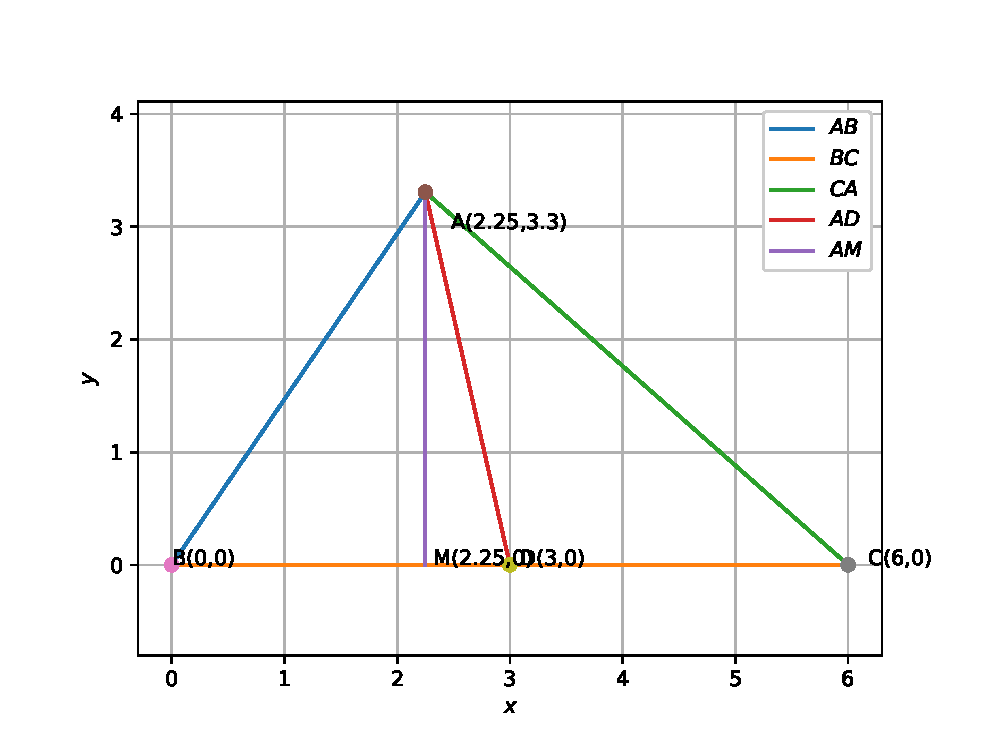
\includegraphics[width=0.8\columnwidth]{./figs/tri_median.eps}
	\end{center}
	\caption{}
	\label{}	
\end{figure}
\end{frame}
\begin{frame}{}
\begin{figure}[!ht]
	\begin{center}
		\resizebox{0.6\columnwidth}{!}{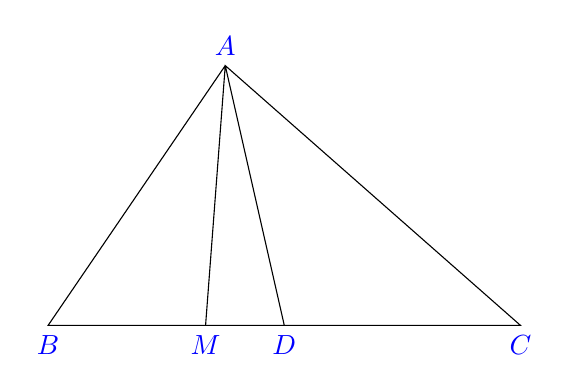
\begin{tikzpicture}[scale=1]

%Triangle sides
\def\a{2.25}
\def\b{3}
\def\c{6}
\def\d{2}
\def\e{3.3}
%Marking coordiantes
\color{blue}
\coordinate [label=above:$A$] (A) at (\a,\e);
\coordinate [label=below:$B$] (B) at (0,0);
\coordinate [label=below:$C$] (C) at (\c,0);
\coordinate [label=below:$D$] (D) at (\b,0);
\coordinate [label=below:$M$] (M) at (\d,0);

%Drawing triangle ABC
\color{black}
\draw (A) -- node[right] {$\textrm{}$} (B) -- node[below] {$\textrm{}$} (C) -- node[right,,xshift=2mm] {$\textrm{}$} (A)-- node[below] {$\textrm{}$} (M) (A)-- node[below] {$\textrm{}$} (D);

%Drawing and marking angles
\tkzMarkRightAngle[fill=blue!20,size=.3](A,M,B)
\tkzLabelAngle[pos=0.65](A,M,B){$ $}
\tkzMarkRightAngle[fill=blue!20,size=.3](A,M,C)
\tkzLabelAngle[pos=0.65](A,M,C){$ $}

\end{tikzpicture}
}
	\end{center}
	\caption{}
	\label{}	
\end{figure}
\end{frame}
\begin{frame}
\textbf{Coordinates of Triangle:}
\begin{enumerate}

\item Construct a $\Delta$ABC with median D and AM $\perp$ BC with a = 2.25, b = 3.3, c = 6 and D = $\frac{B+C}{2}$ = $\begin{pmatrix} 3\\0 \end{pmatrix}.$
\item  AM is the altitude of $\Delta$ABC.\\
\item A = $\begin{pmatrix} b\\a \end{pmatrix}$, B = $\begin{pmatrix} 0\\0 \end{pmatrix}$, C = $\begin{pmatrix} c\\0 \end{pmatrix}$ 
\end{enumerate}
\url{https://github.com/Narendrapulipati/geometry/blob/master/codes/tri_median.py}
\url{https://github.com/Narendrapulipati/geometry/blob/master/figs/tri_median.tex}
\end{frame}
